%====================================================================

%FIGURE: width of likelihood propto 1/sqrt(N)

\begin{figure}[!htbp]
\plotone{figs/sqrtNiso_Stddev_Vs_N.eps}
\caption{The width of the \pdf{} (see Equation \ref{eq:prob}) for two fit parameters found from analyses of 132 mock data sets vs. the number of stars in each data set. (The mock data was created according to the model parameters given in Test \ref{test:sqrtNiso} in Table \ref{tbl:tests}.) The relative standard error (SE) was found from a Gaussian fit to the marginalized \pdf{} for each model parameter. As can be seen, for large data samples the width of the \pdf{} scales with $1/\sqrt{N_{*}}$ as predicted by the central limit theorem.} 
\label{fig:sqrtNiso}
\end{figure}

%====================================================================

%====================================================================

%FIGURE: central limit theorem is satisfied

\begin{figure}[!htbp]
\centering
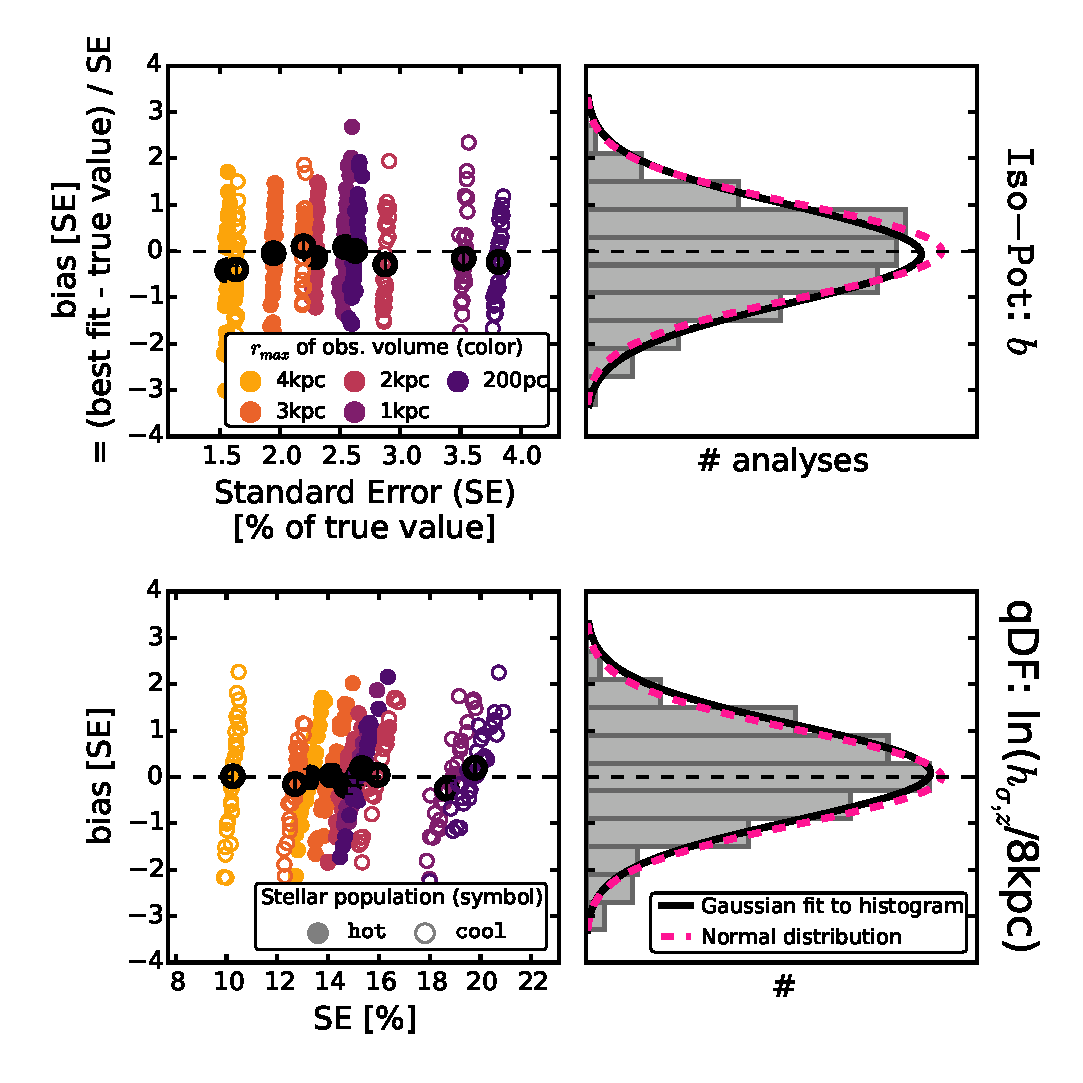
\includegraphics[width=\columnwidth]{figs/isoSph_CLT_2.eps}
\caption{(Un-)bias of the parameter estimates: According to the central limit theorem the the best fit values for a large number of data sets, each containing a large number of stars, will follow the Normal distribution. To test this, we create 320 mock data sets, which come from two different stellar populations and five spherical observation volumes (see legends). (All model parameters are summarized in Table \ref{tbl:tests} as Test \ref{test:isoSph_CLT}.) Bias and relative standard error (SE) are derived from the marginalized \pdf{} for one potential parameter (isochrone scale length $b$ in first row) and one qDF parameter ($h_{\sigma,z}$ in second row). The second column displays a histogram of the 320 offsets. As it closely follows a Normal distribution, our modelling method is therefore well-behaved and unbiased. The black dots show the mean offset and SE for the 32 analyses belonging to one model.}
\label{fig:isoSph_CLT}
\end{figure}

%====================================================================


\subsection{Fitting Procedure} \label{sec:fitting}

To search the $(p_\Phi,p_\text{DF})$ parameter space for the maximum of the \pdf{} in Equation \ref{eq:normalisation}, we go beyond the single fixed grid search by BR13 and employ an effective two-step procedure: Nested-grid search and Monte-Carlo Markov Chain (MCMC).\\

The first step employs a nested-grid search to find the approximate peak and width of the \pdf{} in the high-dimensional \pmodel{}  space at a low number of likelihood evaluations.
\begin{itemize}
\item \emph{Initialization.} For $N_p$ free model parameters \pmodel{}, we start with a sufficiently large grid with $3^N_p$ regular points.

\item  \emph{Evaluation.} We evaluate the \pdf{} at each grid-point similar to BR13 (their Figure 9):  An outer loop iterates over the potential parameters $p_\Phi$ and pre-calculates all $N_* \times N_\text{error} + N_x^2 \times N_v^3$ actions (\# stars times \# MC samples for error convolution, plus actions required for density interpolation grid in Equation \ref{eq:tracerdensity}). Then an inner loop evaluates Equation \ref{eq:normalisation} for all DF parameters $p_\text{DF}$ in the given potential.

\item \emph{Iteration.} For each of the model parameters \pmodel{}, we marginalize the \pdf{}. A Gaussian is fitted to the marginalized \pdf{} and the peak $\pm ~ 4$ sigma become the boundaries of the next $3^{N_p}$ grid. The grid might be still too coarse or badly positioned to fit Gaussians. In that case, we either zoom into the grid point with the highest probability or shift the current range to find new approximate grid boundaries. We proceed with iteratively evaluating the \pdf{} on finer and finer grids, until we have found a reliable 4-sigma fit range in each of the \pmodel{} dimensions. The central grid point is then very close to the best fit \pmodel{}, and the grid range is of the order of the \pdf{} width.

\item \emph{The fiducial qDF.} To save time by pre-calculating actions, they have to be independent of the choice of $p_\text{DF}$. However, the normalisation in Equation \ref{eq:normalisation} requires actions on a $N_x^2 \times N_v^3$ grid and the grid range in velocity space \emph{do} depend on the current $p_\text{DF}$ (see Equation \ref{eq:tracerdensity}). To relax this, we follow BR13 and use a fixed set of qDF parameters (the \emph{fiducial qDF}) to set the velocity grid boundaries in Equation \ref{eq:tracerdensity} globally for a given $p_\Phi$. Choosing a fiducial qDF that is very different from the true DF can however lead to large biases in the \pmodel{} recovery. BR13 did not account for that. \RM{} avoids this as follows: To get successively closer to the optimal fiducial qDF---the (yet unknown) best fit $p_\text{DF}$---we use in each iteration step of the nested-grid search the central grid point of the current \pmodel{} grid as the fiducial qDF.  As the nested-grid search approaches the best fit values, the fiducial qDF approaches its optimum as well. 

\item \emph{Computational expense.} Overall the computation speed of this nested-grid approach is dominated (in descending order of importance) by a) the complexity of potential and action calculation, b) the $N_* \times N_\text{error} + N_x^2 \times N_v^3$ actions required to be calculated per $p_\Phi$, c) the number of potential parameters and d) the number of DF parameters.
\end{itemize}

The second step samples the shape of the \pdf{} using a Monte-Carlo Markov Chain (MCMC). Formally, calculating the \pdf{} on a fine grid like BR13 (e.g. with $K=11$ grid points in each dimension) would provide the same information. However the number of expensive \pdf{} evaluations scales as $K^{N_p}$. For a high-dimensional \pmodel{} ($N_p>4$), a MCMC approach might sample the \pdf{} much faster: We use \emph{emcee} by \citet{2013PASP..125..306F} and release the walkers very close to the best fit \pmodel{} found by the nested-grid search, which assures fast convergence in much less than $K^{N_p}$ \pdf{} evaluations. We also use the best fit \pmodel{} of the grid-search as fiducial qDF for the whole MCMC. In doing so, the normalisation varies smoothly with different $\pmodel{}$ and is slightly less sensitive to the accuracy in Equation \ref{eq:tracerdensity}.